\begin{title}
	Тригонометрическая запись комплексного числа
\end{title}

Декартова или прямоугольная система координат удобна для
графических изображений двумерных векторов. \\
\kv {Горизонтальная ось - действительная} \\
\kv {Вертикальная ось - мнимая (пишут значение i)} \\

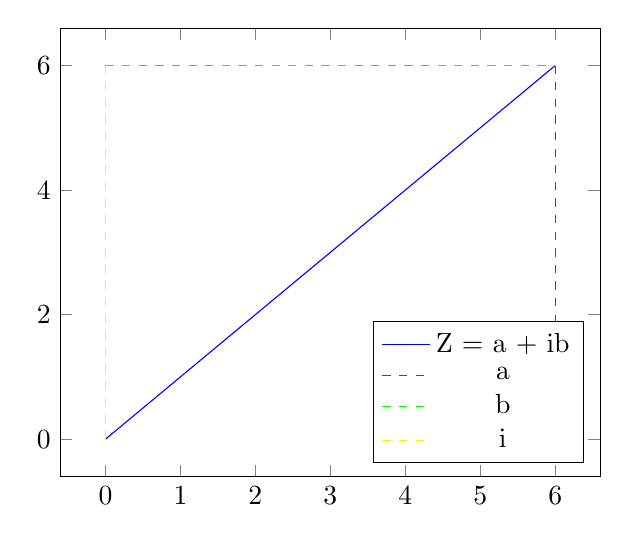
\begin{tikzpicture}
\begin{axis}[legend pos = south east]
\legend{Z = a + ib, a, b, i}
\addplot [solid, draw = blue] coordinates {
	(0,0) (6,6)
};

\addplot [dashed, draw = red] coordinates {
(6,0) (6,6)
};

\addplot [dashed, draw = green] coordinates {
(0,6) (6,6)
};

\addplot [dashed, draw = yellow] coordinates {
(0,0) (0,6)
};

\end{axis}
\end{tikzpicture}

$Z = a + ib \\
Z = (a; b)$ - векторное представление \\
В декартовой системе координат хорошо моделировать сложение
комплексных чисел (сложение векторов) \\

\begin{defin}
	Полярная система координат называется направленный луч, с
	началом в точке \kv
	{О}, которое называется началом координат. \\
	Если \kv {Z} - точка, то она определяется углом $\varphi$,
	который отсчитывается от оси против часовой стрелки $\varphi \in [0;
	2 \Pi]$ и длиной
	радиуса вектора $\rho$. \\
	В итоге точка координат определяется $(\varphi, \rho)$
\end{defin}

Чтобы установить связь между полярной и декартовой системой
координам, совместим на рисунке обе системы координат \\

Пусть даны полярные координаты. Выразим через низ декартовые
координаты. \\
$a = \rho \cdot cos\varphi$ \\
$b = \rho \cdot sin\varphi$ \\
Триганометрическая запись комплексного числа
$Z = \rho (cos\varphi + i \cdot sin \varphi)$ \\
Пусть даны декартовые координаты, выразим полярные. \\
$Z = a + ib \\
\rho = \sqrt{a^2 + b^2} \\
sin \varphi = \frac {b}{\sqrt{a^2 + b^2}} \\
\varphi = arcsin \frac {b}{\sqrt{a^2 + b^2}}$ \\

\bk {Также необходимо знать, чему равен косинус, чтобы
определить в какой четверти лежит угол} \\

\bd {\large {Применение геометрической записи}} \\
\[Z_{1} = \rho_{1} (cos\varphi_{1} + isin\varphi_{1})\] \\
\[Z_{2} = \rho_{2} (cos\varphi_{2} + isin\varphi_{2}\] \\
\[Z_{1} \cdot Z_{2} = \rho_{1} \cdot \rho_{2}
(cos\varphi_{1} \cdot cos\varphi_
{2} - sin\varphi_{1} \cdot sin\varphi_{2} + i(cos\varphi_{1}
\cdot sin\varphi{2}
+ cos\varphi_{2} \cdot sin\varphi_{1})) = \] \\
\[ = \rho_{1} \cdot \rho_{2} (cos(\varphi_{1} + \varphi_{2})
+ i \cdot sin
(\varphi_{1} + \varphi_{2})\] \\

\bd {\large {Геометрический смысл умножения}} \\
\bk{При умножении комплексных числе - их модули
перемножаются, а углы складываются.} \\
Допустим мы хотим найти степени комплексного числа \\
$Z = \rho(cos\varphi + isin\varphi) \\
Z + a + ib \\
Z^n = (a + ib)^n = Z^n = \rho (cos\varphi + isin\varphi)^n =
\rho^n(cos\varphi + isin\varphi)$ \\

$\sqrt[n]{Z} = \sqrt[n]{a + ib}$ - при извлечении корней
декартовые координаты также бесполезны как и при возведении в степень \\
$\sqrt[n]{Z} = \sqrt[n]{\rho}(\sqrt[n]{cos\varphi + isin\varphi}$ \\

Так как $\rho$ - положительное действительное число, то под корнем понимается
таже положительное действительное число, которое принятоназывать
арифметическим.\\
$Z_{1} = cos\psi + isin\psi$ \\
$Z_{1}^n = cos\varphi + isin\varphi$ \\
$n\psi = \varphi \Rightarrow \psi = \frac{\varphi}{n}$ \\

Так как sin и cos периодические, и период равен $2\Pi$, то
кроме этого базовогомрешения бедет еще $n - 1$ решение \\
$\psi = \frac {\varphi + 2\Pi k}{n}$ \\
$k = 0, 1, 2 ... n - 1$ \\

От сюда выводится \bd {формула Демуавра} \\
$\sqrt[n]{Z} = \sqrt[n]{\rho} (cos\psi + isin\psi)$ \\
$\psi = \frac {\varphi + 2\Pi k}{n} ~~ k = 0, 1, 2 ... n -1$ \\

\bk {Замечание} \\
Корни n-ной стемени из единицы - являются вершинами
правильного многоугольника, у которого начальная вершина
имеет координаты (1; 0) \\

\begin{defin}
	Поле \kv {P} - алгебраически замкнуто, если любой многочлен с
	коэффициентом в этом поле разлагается на линейные множители.
          То есть имеет хотя бы один корень.
\end{defin}

\begin{defin}
	\kv {P} - Алгебраически замкнуто, если любой многочлен с коэффициентами в этом
	поле, имеет хотя бы один корень в этом поле.
\end{defin}

\begin{theorem}
           Всякий многочлен положительной степени над полем комплексных чисел имеет корень.
\end{theorem}

Из этой теоремы и определения алгебраической замкнутости выходит основная теорема алгебры.\\
\begin{theorem}[Основная теорема алгебры]
	Поле комплексных чисел, является алгебраически замкнутым.
\end{theorem}

\begin{defin}
	Расширение поля \bk{Р} до поля \bk{F} называется алгебраическим, если любой
	элемент поля \bk {F} является корнем некоторого многочлена с коэффициентом из
	поля \bk {P}.\\
	У поля комплексных чисел нет алгебраических расширений.
\end{defin}

\begin{title}
	Теория многочленов (полиномов)
\end{title}

Пусть \bk{P} - поле. $P[x]$ - кольцо многочленов. Как мы знаем - это кольцо
Евклидово с Евклидовой нормой, равной многочлену \bk{f(x)}. \\
$\rho (f(x)) = степень f(x)$ \\
Была доказана теорема, что это кольцо с однозначным разложением на простые
множетели. \\
Простыми элементам называются неприводимые многочлены. \\
Можно взять $x_{1}, x_{2}, ... x_{n} ~~ P[x_{1} ... x_{n}]$ и рассмотреть кольцо
многочлена от \kv {n} элементов. \\
$\sum_{i_{1}...i_{n}}^k a_{i_{1}...i_{n}} x_{1}^{i_{1}} ... x_{n}^{i_{k}}$ \\
$P \to P[x_{1}] \to (P[x_{1}])[x_{2}$ - тоже самое, что и $P[x_{1} ... x_{2}]$\\

Так как множество многочленов образует кольцо, то нужно ввести некоторые
понятия, актуальные для всех колец \\

\bk {1-е понятие} \\
\kv {Гомоморфизм и Изоморфизм} \\
Пусть $G - * ~~ H - \circ$ - 2 группы \\
$\varphi: G \to H$ - \kv {гомоморфизм групп} \\
Если $\forall q_{1},q_{2} \in G ~~ \varphi(g_{1} * g_{2}) = \varphi(g_{1}) \circ
\varphi(g_{2})$ \\
Содержательно гоморфизм сохраняет операцию, образ результата умножения равен
произведению образа.\\
Отображение называется гомоморфизмом групп, если оно одну групповую операцию
переводит в другую. Но обратно вернуться нельзя, другая операция не может уже
перейти в первую операцию.\\
А если можно в обе стороны, то это уже изоморфизм групп. 
То есть первая операция переходит во вторую, а вторая
опять может перейти в первую.\\

Пусть $K - (+*) ~~ L - (\oplus \circ)$ \\
$\varphi: K \to L$ - \kv {гомоморфизм колец} \\
Если $\forall k_{1}, k_{2} \in K ~~ \varphi(k_{1} + k_{2}) = \varphi(k_{1})
\oplus \varphi(k_{2}) ~~ \varphi(k_{1} * k_{2}) = \varphi(k_{1}) \circ
\varphi(k_{2})$ \\
Гомоморфизм колец сохраняет обе операции. \\

\begin{defin}
Если отображение $\varphi$ - является биекцией, то гомоморфизм $\varphi$ -
изоморфизм.
\end{defin}

Биекция сохряняет все элементы при отображении, следовательно гомоморфизм
становиться изоморфизмом.\\
Гомоморфизм - интерпритация одних объектов и их отношений в терминах других
объектов и других отношений. \\
